% =====================================================================
%  Assignment 3 Report -- Data Science for Software Engineering
%  Full, self-contained, compilable source (reconstructed + Week 2/3 added).
%  Build:  tectonic report.tex     (or: latexmk -pdf report.tex)
% =====================================================================
\documentclass[11pt,a4paper]{report}

\usepackage[utf8]{inputenc}
\usepackage[T1]{fontenc}
\usepackage[a4paper,margin=2.5cm]{geometry}
\usepackage{booktabs}
\usepackage{graphicx}
\usepackage{amsmath}
\usepackage{float}
\usepackage{caption}
\usepackage[hidelinks]{hyperref}

% Figures are produced by the analysis scripts under data/outputs/.
\graphicspath{{data/outputs/}{data/outputs/week2/}{data/outputs/week3/}}

\title{\vspace{3cm}\Huge\bfseries Assignment 3 Report\\[0.5em]
       \large\mdseries Data Science for Software Engineering}
\author{Brian Stevo Aranha \and Achara Obinna Vincent \and
        Namit Joshi \and Anil Kumar}
\date{July 4, 2026}

\begin{document}

% ---- Title page --------------------------------------------------------
\begin{titlepage}
  \centering
  \vspace*{2cm}
  {\Large\scshape Universit\"at Paderborn\par}
  \vspace{3cm}
  {\Huge\bfseries Assignment 3 Report\par}
  \vspace{0.6cm}
  {\Large Data Science for Software Engineering\par}
  \vspace{3cm}
  {\large
   Brian Stevo Aranha\\
   Achara Obinna Vincent\\
   Namit Joshi\\
   Anil Kumar\par}
  \vspace{1.5cm}
  {\large July 4, 2026\par}
  \vfill
\end{titlepage}

\tableofcontents

% =======================================================================
\chapter{Introduction}
\section{Introduction}
Issue tracking systems such as Jira contain useful software engineering
discussions about bugs, improvements, features and design decisions. Prior work
has shown that bug reports provide important information for developers, although
the quality and completeness of this information can vary~\cite{bettenburg}. In
this task, we focus on Apache Tika issues from the Apache Jira issue
tracker~\cite{tika}. The overall goal is to explore the \emph{topics} of design
issues using topic modeling (LDA and BERTopic) and to study their
characteristics and their co-occurrence with three types of design decisions:
\emph{existence}, \emph{property} and \emph{executive}.

% =======================================================================
\chapter{Study Design}
We used the \texttt{Tika} sheet from the provided Excel file because Apache Tika
is our selected project. The sheet contained 211 issue IDs and three
design-decision labels: existence, property and executive.

Using Python, we downloaded the corresponding issue data from Apache Jira. The
downloaded fields included summary, description, issue type, status, resolution,
priority, labels, components, dates, parent issue, number of comments and number
of attachments.

For preprocessing, we combined each issue summary and description into one text
field. The text was cleaned by lowercasing, removing URLs and special
characters, splitting camel-case words, removing stop words, lemmatizing tokens
and removing very short tokens.

For Week~2, Latent Dirichlet Allocation (LDA) topic modeling was applied in two
iterations using the Gensim library~\cite{gensim}. In both iterations the model
parameters were $\alpha=0.01$, $\beta=0.01$, 20 training passes, 400 iterations
per pass, and a fixed random seed of 50. The low symmetric $\alpha$ encourages
sparse topic distributions so that each issue is strongly associated with one
dominant topic. Iteration~1 used a fixed number of 10 topics. To find the
optimal number of topics, $C_V$ coherence scores were computed for $k=1$ to
$k=10$, and the $k$ with the highest coherence was selected for Iteration~2. For
Iteration~2, each token was replaced with its ontology class label
(\texttt{COMPONENT}, \texttt{CONNECTOR}, \texttt{DATA}, \texttt{SOLUTION},
\texttt{TECHNOLOGY}, \texttt{QUALITY\_ATTRIBUTE}) where it appeared in the
ontology, and LDA was re-run with the optimal $k$.

The second topic model, BERTopic~\cite{bertopic}, was run on the same
preprocessed text using \texttt{all-MiniLM-L6-v2} sentence
embeddings~\cite{sbert}. Because the small corpus is dominated by one dense
cluster, the default HDBSCAN clustering produced only two topics; we therefore
used KMeans ($k=7$, matching the LDA optimum) so that BERTopic yields a
comparable, balanced set of topics with every issue assigned.

For Week~3 we analysed the issues of each topic. Numeric issue characteristics
(comments, attachments, description length, token count) were compared across
topics with Kruskal--Wallis tests and Dunn post-hoc tests; issue type was
compared with $\chi^2$ tests. Co-occurrences between LDA topics, BERTopics and
the three decision types were tested with $\chi^2$ tests, standardized
residuals, and Fisher exact tests with Benjamini--Hochberg correction.

% =======================================================================
\chapter{Results}

\section{Week 1: Issue Data Download and Vocabulary Creation}
A total of 211 Apache Tika issues were processed. All issues were successfully
downloaded from Jira using the provided issue list. For each issue, the summary,
description, issue type, status, priority, parent-issue information, number of
comments and number of attachments were collected. As expected, most issues have
no parent: only 10 of the 211 issues (4.7\%) reference a parent issue.

After downloading, the issue summary and description were combined and
preprocessed. After preprocessing, no issue had zero tokens; the average number
of tokens per issue was 69.78. The vocabulary contained 14{,}724 total tokens
and 2{,}706 unique tokens. The most frequent tokens included \texttt{parser},
\texttt{file}, \texttt{metadata}, \texttt{type}, \texttt{text}, \texttt{content},
\texttt{test}, \texttt{code}, \texttt{document}, \texttt{version}, \texttt{pdf},
\texttt{user}, \texttt{server}, \texttt{stream}, \texttt{data}, \texttt{parse},
\texttt{class}, \texttt{java}, \texttt{vulnerability} and \texttt{cve}. A
document-term matrix of shape $211\times2706$ was created and used as input for
LDA (Figure~\ref{fig:top20}).

\begin{figure}[H]
  \centering
  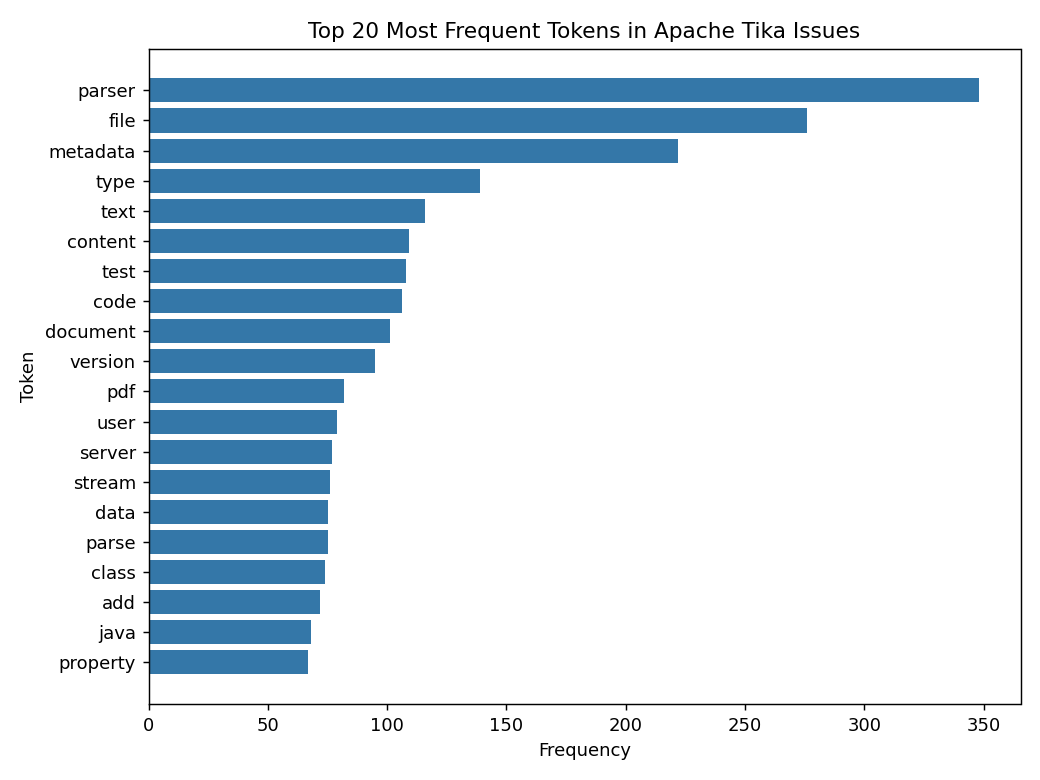
\includegraphics[width=0.75\textwidth]{tika_top20_tokens.png}
  \caption{Top 20 most frequent tokens in the preprocessed Apache Tika issues.}
  \label{fig:top20}
\end{figure}

\section{Week 2: LDA Topic Modeling}

\subsection*{Iteration 1: 10 topics}
LDA was trained on the 211 preprocessed issues with 10 topics.
Table~\ref{tab:lda1} lists the top three terms, the number of assigned issues
and a brief theme for each topic. Topic~8 was the largest group with 51 issues,
covering the core parser API. Topic~4 captured dependency-vulnerability reports
(Sonatype, jar files, CVE). Most issues received a dominant-topic probability
above 0.99, reflecting the sparse distribution produced by the low $\alpha$.

\begin{table}[H]
  \centering
  \caption{Iteration 1: top terms per topic (10 topics, $\alpha=\beta=0.01$).}
  \label{tab:lda1}
  \begin{tabular}{clrl}
    \toprule
    \textbf{Topic} & \textbf{Top 3 terms} & \textbf{Issues} & \textbf{Theme} \\
    \midrule
    0 & metadata, code, name       & 22 & Metadata and EXIF \\
    1 & file, text, parser         & 21 & File and content parsing \\
    2 & image, embedded, content   & 13 & Image and OCR \\
    3 & metadata, mapping, java    & 11 & Metadata mapping \\
    4 & file, sonatype, java       & 26 & Dependency vulnerabilities \\
    5 & document, file, parser     & 18 & Document parsing \\
    6 & test, pdf, file            & 16 & PDF testing \\
    7 & log, file, version         & 19 & Logging and CVE \\
    8 & parser, metadata, content  & 51 & Parser API \\
    9 & parser, file, content      & 14 & Content and configuration \\
    \bottomrule
  \end{tabular}
\end{table}

\subsection*{Coherence analysis}
$C_V$ coherence scores were computed for $k=1$ to $k=10$
(Table~\ref{tab:coh}, Figure~\ref{fig:coh}). The score peaked at $k=7$
($C_V=0.3462$), which was used for Iteration~2.

\begin{table}[H]
  \centering
  \caption{$C_V$ coherence scores for $k=1$ to $k=10$.}
  \label{tab:coh}
  \begin{tabular}{cc}
    \toprule
    $k$ & $C_V$ coherence \\
    \midrule
    1 & 0.2228 \\ 2 & 0.2270 \\ 3 & 0.2539 \\ 4 & 0.2611 \\ 5 & 0.3156 \\
    6 & 0.3420 \\ \textbf{7} & \textbf{0.3462} \\ 8 & 0.3299 \\ 9 & 0.3268 \\
    10 & 0.3313 \\
    \bottomrule
  \end{tabular}
\end{table}

\begin{figure}[H]
  \centering
  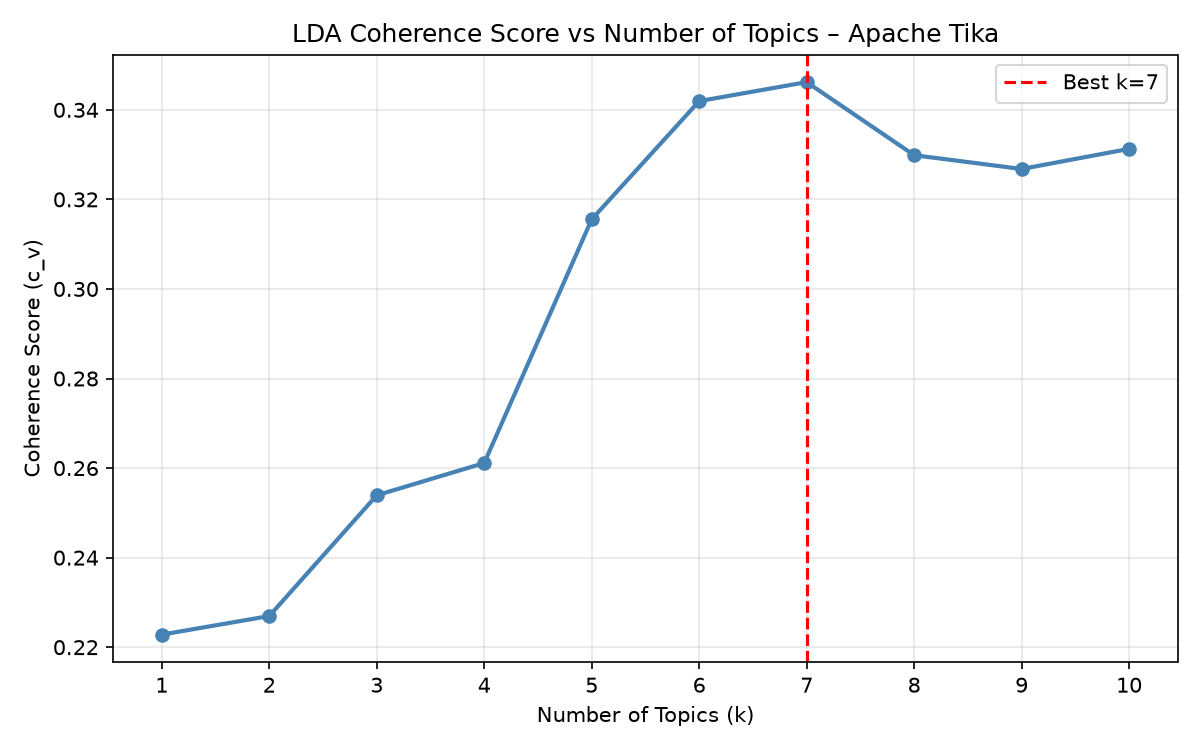
\includegraphics[width=0.7\textwidth]{lda_coherence_scores.png}
  \caption{$C_V$ coherence score for $k=1$ to $k=10$. The highest value is at
           $k=7$.}
  \label{fig:coh}
\end{figure}

\subsection*{Iteration 2: ontology replacement}
Before re-running LDA, tokens that appeared in the ontology were replaced with
their class labels. A total of 2{,}832 replacements were made across all 211
issues. LDA was then trained with $k=7$ (Table~\ref{tab:lda2}). The class label
\texttt{COMPONENT} appeared as a top term in all seven topics, reflecting that
most issues involve software components. Topic~4 was the largest (89 issues),
covering the general parser framework; Topic~3 was the most distinct, capturing
security vulnerabilities (\texttt{vulnerability}, \texttt{cve},
\texttt{sonatype}).

\begin{table}[H]
  \centering
  \caption{Iteration 2: top terms per topic with ontology replacement ($k=7$).}
  \label{tab:lda2}
  \begin{tabular}{clr}
    \toprule
    \textbf{Topic} & \textbf{Top 3 terms} & \textbf{Issues} \\
    \midrule
    0 & TECHNOLOGY, DATA, COMPONENT       & 17 \\
    1 & COMPONENT, TECHNOLOGY, DATA       & 63 \\
    2 & property, log, COMPONENT          &  9 \\
    3 & COMPONENT, version, vulnerability & 21 \\
    4 & COMPONENT, parser, CONNECTOR      & 89 \\
    5 & test, pdf, COMPONENT              &  4 \\
    6 & memory, text, DATA                &  8 \\
    \bottomrule
  \end{tabular}
\end{table}

\section{Week 2: BERTopic Topic Modeling}
BERTopic was run on the 211 preprocessed issues using \texttt{all-MiniLM-L6-v2}
sentence embeddings. The default HDBSCAN clustering collapsed the corpus into
only two topics (178 and 33 issues), too coarse to compare with LDA or to test
co-occurrences. We therefore replaced the clustering step with KMeans ($k=7$),
yielding seven balanced, interpretable topics with every issue assigned and no
outliers (Table~\ref{tab:bert}); a fixed random state of 42 makes the run
reproducible. Compared with LDA, BERTopic produced a more even distribution
(17--44 issues per topic versus LDA's 4--89) and kept the vulnerability topic
(Topic~2) sharply separated.

\begin{table}[H]
  \centering
  \caption{BERTopic topics ($k=7$): top terms, number of issues, and theme.}
  \label{tab:bert}
  \begin{tabular}{clrl}
    \toprule
    \textbf{Topic} & \textbf{Top terms} & \textbf{Issues} & \textbf{Theme} \\
    \midrule
    0 & test, pdf, type, image, file      & 44 & File-type detection / PDF \& image \\
    1 & metadata, property, field, parser & 35 & Metadata extraction \\
    2 & version, vulnerability, log, jar  & 33 & Dependency \& security vulnerabilities \\
    3 & parser, metadata, document, file  & 31 & Document parsing \& configuration \\
    4 & parser, java, microsoft, parse    & 29 & Office / language-specific parsers \\
    5 & file, server, url, fetcher        & 22 & Tika-server \& fetchers \\
    6 & process, stream, input, processor & 17 & Streaming / async processing \\
    \bottomrule
  \end{tabular}
\end{table}

\section{RQ1: Topics and Keywords from LDA and BERTopic}
\emph{What topics emerge from LDA and BERTopic and what are the common keywords
per topic?} Both algorithms surface the same broad areas of Apache Tika: a large
parser/metadata core, document/PDF/image handling, the tika-server, and a
distinct security and dependency-vulnerability topic (LDA Topic~3; BERTopic
Topic~2). LDA (after ontology replacement) is dominated by one large topic
(Topic~4, 89 issues) and relies heavily on the abstract ontology labels, whereas
BERTopic gives a more balanced and more concrete keyword picture (e.g.\
\texttt{microsoft}, \texttt{fetcher}, \texttt{image}, \texttt{vulnerability}).
The number of issues per topic is reported in Tables~\ref{tab:lda2}
and~\ref{tab:bert}.

\section{Week 3: Characteristics and Co-occurrences}

\subsection{RQ2: Characteristics of the issues in each topic}
For each topic we compared four numeric characteristics---number of comments,
number of attachments, description length (characters) and preprocessed token
count---using Kruskal--Wallis omnibus tests (the count fields are strongly
right-skewed), followed by Dunn post-hoc tests where the omnibus test was
significant. Issue type was compared with a $\chi^2$ test.

\begin{table}[H]
  \centering
  \caption{Kruskal--Wallis omnibus tests for issue characteristics per topic.}
  \label{tab:rq2}
  \begin{tabular}{llrrc}
    \toprule
    \textbf{Model} & \textbf{Characteristic} & \textbf{H} & \textbf{p} & \textbf{Sig.}\\
    \midrule
    LDA      & comments           & 2.35  & 0.885    & no \\
    LDA      & attachments        & 2.76  & 0.838    & no \\
    LDA      & description length & 4.58  & 0.599    & no \\
    LDA      & token count        & 4.71  & 0.582    & no \\
    \midrule
    BERTopic & comments           & 7.09  & 0.312    & no \\
    BERTopic & attachments        & 35.35 & $<0.001$ & \textbf{yes} \\
    BERTopic & description length & 14.65 & 0.023    & \textbf{yes} \\
    BERTopic & token count        & 13.81 & 0.032    & \textbf{yes} \\
    \bottomrule
  \end{tabular}
\end{table}

LDA topics do \emph{not} separate issues by any metadata characteristic (all
$p>0.27$). BERTopic topics do: they differ significantly in attachments,
description length and token count, though not in comments. The vulnerability
topic (BERTopic Topic~2) has the longest, most detailed descriptions. Issue type
is also strongly associated with BERTopic topic ($\chi^2=164$, $p<0.001$;
Figure~\ref{fig:rq2type}). We note that $67\%$ of the expected cell counts here
are below five, so this $\chi^2$ is approximate and should be read together with
the heatmap.

\begin{figure}[H]
  \centering
  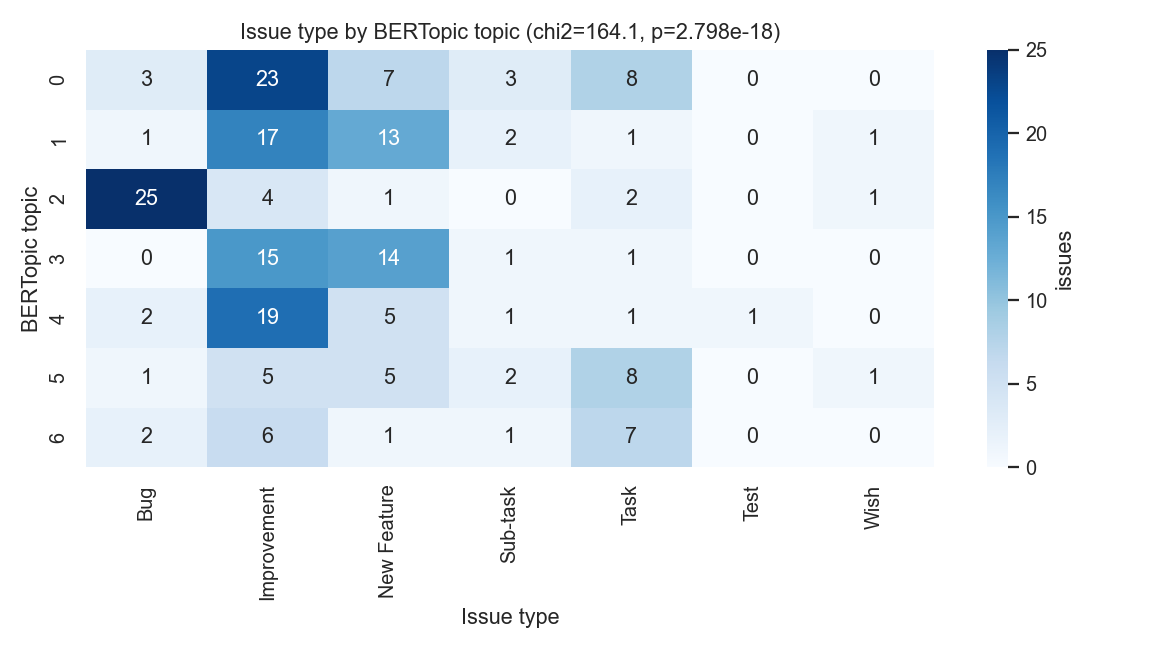
\includegraphics[width=0.8\textwidth]{rq2_issue_type_BERTopic.png}
  \caption{Issue type by BERTopic topic.}
  \label{fig:rq2type}
\end{figure}

\subsection{RQ3: Co-occurrences}

\subsubsection*{(a) LDA topics versus BERTopics}
The $7\times7$ contingency table of LDA versus BERT topic assignments is
significantly associated ($\chi^2=114.9$, $\mathrm{dof}=36$,
$p=3.6\times10^{-10}$). Standardized residuals identify six topic pairs that
co-occur more or less than chance. The strongest is \textbf{LDA Topic~3
$\leftrightarrow$ BERT Topic~2} (residual $=5.9$): both are the
security/vulnerability topic, i.e.\ the two models independently isolate the same
issues (Figure~\ref{fig:rq3cross}). As above, $71\%$ of expected cells are below
five, so the omnibus $\chi^2$ is approximate and the residual pattern is reported
as descriptive evidence of alignment.

\begin{figure}[H]
  \centering
  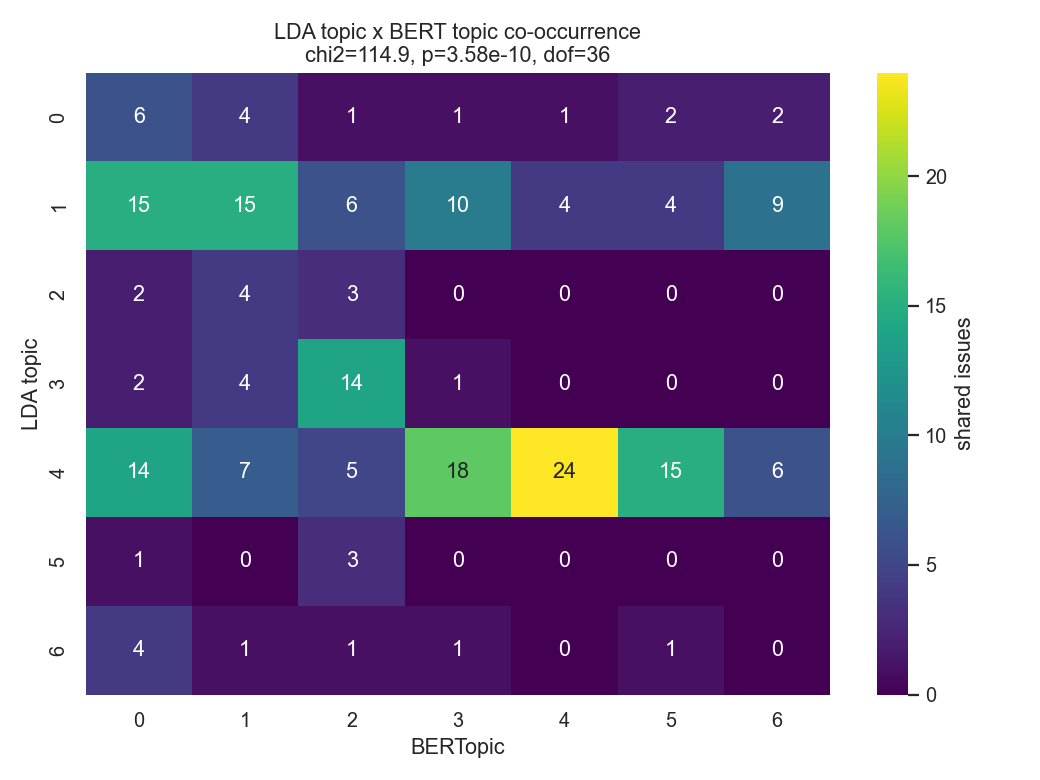
\includegraphics[width=0.65\textwidth]{rq3_lda_vs_bert_heatmap.png}
  \caption{Issues shared between each LDA topic (rows) and BERTopic (columns).}
  \label{fig:rq3cross}
\end{figure}

\subsubsection*{(b) Topics versus the three design-decision types}
Each issue belongs to one topic but may carry several decision types, so for
every (topic, decision) pair we ran a Fisher exact test (odds ratio) and
corrected $p$-values within each model with Benjamini--Hochberg
(Table~\ref{tab:rq3fisher}). The security topic (BERTopic Topic~2 / LDA Topic~3)
is overwhelmingly associated with \textbf{property} and \textbf{executive}
decisions and essentially never an \textbf{existence} decision: dependency
upgrades and vulnerability fixes change \emph{how} something is done or
\emph{which} technology is used, not \emph{whether} a component exists.
Conversely, the metadata and document-parsing topics (BERTopic~1,~3) and the
parser-core topic (LDA~4) are associated with \textbf{existence} decisions
(Figure~\ref{fig:rq3dec}).

\begin{table}[H]
  \centering
  \caption{Significant (FDR $<0.05$) topic $\leftrightarrow$ decision
           associations (selected).}
  \label{tab:rq3fisher}
  \begin{tabular}{cllrrr}
    \toprule
    \textbf{Model} & \textbf{Topic} & \textbf{Decision} & \textbf{\% w/ dec.} &
    \textbf{OR} & \textbf{$p_{\text{adj}}$} \\
    \midrule
    BERTopic & 2 (security)    & property  & 97.0 & 66.2 & $<0.001$ \\
    BERTopic & 2 (security)    & executive & 90.9 & 34.5 & $<0.001$ \\
    BERTopic & 2 (security)    & existence &  6.1 & 0.02 & $<0.001$ \\
    BERTopic & 1 (metadata)    & existence & 88.6 & 4.43 & 0.009 \\
    BERTopic & 3 (doc parsing) & existence & 90.3 & 5.28 & 0.009 \\
    LDA      & 3 (security)    & executive & 76.2 & 8.06 & $<0.001$ \\
    LDA      & 3 (security)    & property  & 71.4 & 3.83 & 0.048 \\
    LDA      & 4 (parser core) & existence & 78.7 & 2.47 & 0.032 \\
    \bottomrule
  \end{tabular}
\end{table}

\begin{figure}[H]
  \centering
  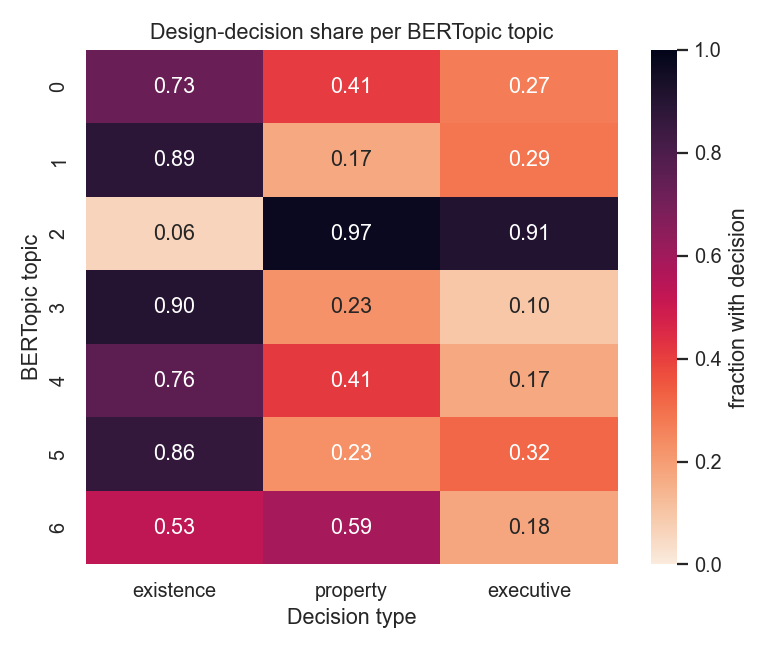
\includegraphics[width=0.5\textwidth]{rq3_BERTopic_decision_heatmap.png}
  \caption{Fraction of each BERTopic topic carrying each design-decision type.}
  \label{fig:rq3dec}
\end{figure}

\subsubsection*{(c) Co-occurrence among the three decision types}
We also tested whether the decision types co-occur with each other
(Table~\ref{tab:rq3dec}). \textbf{Existence} decisions are largely mutually
exclusive with \textbf{property} ($\phi=-0.80$; because every issue has one or
the other, the odds ratio collapses to $\approx0$) and, less strongly, with
\textbf{executive} ($\phi=-0.38$). In contrast, \textbf{property} and
\textbf{executive} decisions tend to co-occur ($\phi=+0.27$, $\mathrm{OR}=3.2$).
Deciding \emph{whether} a component exists is a different kind of decision from
deciding \emph{how} it should behave or \emph{which} technology to use, and the
latter two often travel together (Figure~\ref{fig:rq3deccooc}). Every issue
carries at least one decision type; existence-only is the largest group
($44.5\%$) and property${+}$executive is the most common combination ($19.0\%$).

\begin{table}[H]
  \centering
  \caption{Co-occurrence among the three design-decision types.}
  \label{tab:rq3dec}
  \begin{tabular}{lrrrrl}
    \toprule
    \textbf{Pair} & \textbf{Both} & \textbf{OR} & \textbf{$\phi$} &
    \textbf{$p_{\text{adj}}$} & \textbf{Association} \\
    \midrule
    existence $\leftrightarrow$ property  & 22 & $\approx0$ & $-0.80$ & $<0.001$ & strong negative \\
    existence $\leftrightarrow$ executive & 30 & 0.19       & $-0.38$ & $<0.001$ & negative \\
    property  $\leftrightarrow$ executive & 43 & 3.19       & $+0.27$ & $<0.001$ & positive \\
    \bottomrule
  \end{tabular}
\end{table}

\begin{figure}[H]
  \centering
  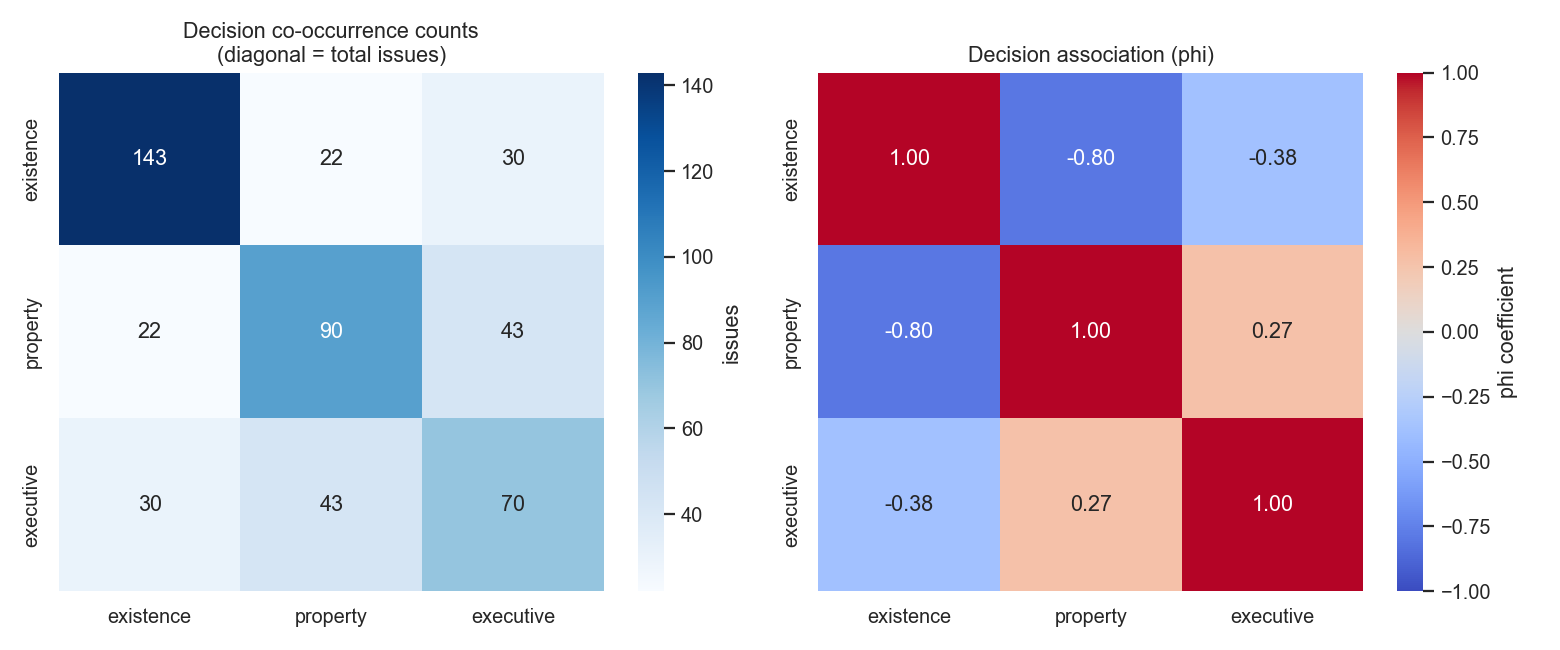
\includegraphics[width=0.85\textwidth]{rq3_decision_cooccurrence_heatmap.png}
  \caption{Left: co-occurrence counts among decision types (diagonal = total
           issues). Right: phi association between decision types.}
  \label{fig:rq3deccooc}
\end{figure}

% =======================================================================
\chapter{Discussion}
The Week~1 preparation was successful: all 211 issues were downloaded and still
had usable text after preprocessing. The most frequent tokens (\texttt{parser},
\texttt{file}, \texttt{metadata}, \texttt{document}, \texttt{pdf},
\texttt{content}) reflect Tika's role in parsing files and extracting text and
metadata, and terms such as \texttt{vulnerability}, \texttt{cve} and
\texttt{vulnerable} already hinted at a security topic.

The LDA results confirmed this. Iteration~1 surfaced two security-related topics
(dependency vulnerabilities and logging/CVE), and the coherence analysis rose
steadily to a peak at $k=7$, indicating that seven is a meaningful granularity.
Ontology replacement in Iteration~2 collapsed many tokens into six class labels;
this surfaced the architectural dimension (the dominance of \texttt{COMPONENT})
but also reduced the discriminative power between topics, leaving Topics~0,~1
and~6 harder to interpret.

BERTopic was more informative once re-tuned. The original two-topic run was too
coarse; the seven-topic KMeans configuration produced balanced, concrete topics
and, unlike LDA, its topics differed significantly in issue characteristics
(RQ2) --- particularly attachments and description length --- and aligned
strongly with LDA on the security topic (RQ3a).

The headline finding (RQ3b) is the sharp division of labour between decision
types and topics: the security topic maps onto \emph{property} and
\emph{executive} decisions, while component-adding topics map onto
\emph{existence}. RQ3c reinforces this at the decision level: existence
decisions are almost mutually exclusive with property, while property and
executive travel together. Together these results suggest that topic membership
is a useful predictor of the \emph{type} of design decision an issue records.

% =======================================================================
\chapter{Threats to Validity}
\section{Internal Validity}
Preprocessing choices (stop-word removal, lemmatization, deletion of short
tokens) affect the vocabulary and therefore the topics. A fixed random seed
makes the models reproducible, but different hyperparameters for $\alpha$,
$\beta$ or the number of passes could change topic assignments. The coherence
optimisation was limited to $k=1$ to $k=10$, so a globally better $k$ could lie
outside this range, and $C_V$ measures statistical co-occurrence of terms rather
than whether topics are meaningful for design decisions.

\section{External Validity}
The study focuses only on Apache Tika, so results may not generalise to other
projects, each of which has its own terminology and issue discussions.

\section{Construct Validity}
Only the issue summary and description were used for text analysis; useful
information in comments or attachments was not included. BERTopic used KMeans
($k=7$) because HDBSCAN under-clustered this small corpus; KMeans forces a fixed
$k$ and assigns every issue, which is convenient for co-occurrence but removes
BERTopic's automatic topic-count selection. Several $\chi^2$ tests have more than
$20\%$ of expected cells below five (flagged as \texttt{pct\_expected\_lt5} in
the output CSVs), so the pairwise conclusions rely on exact Fisher tests, and
Benjamini--Hochberg correction was applied across all topic\,$\times$\,decision
pairs.

% =======================================================================
\chapter{Conclusion and Future Work}
Across the three weeks we prepared the Apache Tika issue dataset, applied two
topic models, and analysed the resulting topics. Week~1 produced a clean corpus,
vocabulary and document-term matrix. Week~2 ran LDA (with a coherence-selected
$k=7$ and an ontology-enriched iteration) and BERTopic, answering RQ1: both
models recover a parser/metadata core, document and image handling, a
tika-server area, and a distinct security topic. Week~3 answered RQ2 and RQ3:
BERTopic topics differ significantly in issue characteristics, topics from the
two models align on the security theme, and topics co-occur meaningfully with
the three decision types---security with property/executive, component work with
existence.

Future work could extend the coherence search beyond $k=10$, incorporate issue
comments into the text, refine the ontology so LDA Iteration~2 stays
interpretable, and validate the topic--decision associations on a second Apache
project to test generalisability.

% =======================================================================
\appendix
\chapter{Team Effort and Contributions}
Tables~\ref{tab:w1}--\ref{tab:w3} summarise the main activities per week. Rows
marked \emph{(to be filled)} are to be completed by the respective team members.

\begin{table}[H]
  \centering
  \caption{Summary of team effort in Week 1.}
  \label{tab:w1}
  \begin{tabular}{p{3cm} c p{9cm}}
    \toprule
    \textbf{Name} & \textbf{Hours} & \textbf{Activities} \\
    \midrule
    Obinna & 6 & Organised the Week~1 folder; processed the Tika issue list and
                 downloaded the Jira issue data; preprocessed summaries and
                 descriptions; created the vocabulary and document-term matrix. \\
    Anil   & 8 & Fetched all issues from the Jira API; applied tokenisation,
                 stop-word removal, lemmatisation and ontology-class replacement;
                 created the filtered vocabulary. \\
    Brian  & -- & \textit{(to be filled)} \\
    Namit  & 0 & No contribution in Week~1. \\
    \bottomrule
  \end{tabular}
\end{table}

\begin{table}[H]
  \centering
  \caption{Summary of team effort in Week 2.}
  \label{tab:w2}
  \begin{tabular}{p{3cm} c p{9cm}}
    \toprule
    \textbf{Name} & \textbf{Hours} & \textbf{Activities} \\
    \midrule
    Brian & 7 & Ran the topic-modeling algorithms (LDA and BERTopic); wrote the
                Week~2 LDA report section. \\
    Namit & 2 & Fixed the BERTopic results: the initial run collapsed into two
                topics, so re-ran BERTopic with KMeans ($k=7$) to obtain seven
                balanced, interpretable topics and the per-issue assignments used
                for the Week-3 co-occurrence analysis. \\
    Obinna & -- & \textit{(to be filled)} \\
    Anil   & -- & \textit{(to be filled)} \\
    \bottomrule
  \end{tabular}
\end{table}

\begin{table}[H]
  \centering
  \caption{Summary of team effort in Week 3.}
  \label{tab:w3}
  \begin{tabular}{p{3cm} c p{9cm}}
    \toprule
    \textbf{Name} & \textbf{Hours} & \textbf{Activities} \\
    \midrule
    Namit  & 9 & RQ2: per-topic characteristics (comments, attachments,
                 description length, tokens) with Kruskal--Wallis and Dunn tests,
                 box plots and issue-type $\chi^2$. RQ3: LDA\,$\times$\,BERT
                 co-occurrence, topic\,$\times$\,decision Fisher tests (FDR) and
                 decision-type co-occurrence. Wrote and integrated the Week-3
                 report sections. \\
    Brian  & -- & \textit{(to be filled)} \\
    Obinna & -- & \textit{(to be filled)} \\
    Anil   & -- & \textit{(to be filled)} \\
    \bottomrule
  \end{tabular}
\end{table}

% =======================================================================
\begin{thebibliography}{9}
\bibitem{tika}
Apache Software Foundation. \emph{Apache Tika Issues on Apache Jira}.
\url{https://issues.apache.org/jira/projects/TIKA/issues}. Accessed 26 June
2026, 2026.

\bibitem{bettenburg}
Nicolas Bettenburg et al. ``What Makes a Good Bug Report?'' In: \emph{Proc.\ 16th
ACM SIGSOFT Int.\ Symp.\ on Foundations of Software Engineering}. FSE-16. ACM,
2008, pp.\ 308--318.

\bibitem{gensim}
Radim \v{R}eh\r{u}\v{r}ek and Petr Sojka. ``Software Framework for Topic
Modelling with Large Corpora''. In: \emph{Proc.\ LREC 2010 Workshop on New
Challenges for NLP Frameworks}. Valletta, Malta: ELRA, 2010, pp.\ 45--50.

\bibitem{bertopic}
Maarten Grootendorst. ``BERTopic: Neural topic modeling with a class-based
TF-IDF procedure''. \emph{arXiv:2203.05794}, 2022.

\bibitem{sbert}
Nils Reimers and Iryna Gurevych. ``Sentence-BERT: Sentence Embeddings using
Siamese BERT-Networks''. In: \emph{Proc.\ EMNLP-IJCNLP}. ACL, 2019.
\end{thebibliography}

\end{document}
